{
\metroset{titleformat frame=smallcaps}
\begin{frame}{Use Case 3: Ransomware Detection at the Network Edge}
      \vspace{7pt}
  \subtitlebar{Moving defense from the user device to the switch --- before the attack arrives}

  \begin{columns}[T, totalwidth=\textwidth]

    % ── Left: 3 Boxes ─────────────────────────────────────
    \begin{column}{0.44\textwidth}

      \begin{tcolorbox}[problemcard=problemred]
        {\color{problemred}\bfseries\scriptsize The Threat}\\[2pt]
        {\footnotesize\color{HUAdark}
        Ransomware hijacks files and extorts money.
        Traditional defenses activate only after
        the attack reaches the device.}
      \end{tcolorbox}

      \vspace{6pt}

      \begin{tcolorbox}[problemcard=HUAblue]
        {\color{HUAblue}\bfseries\scriptsize AI in Action}\\[2pt]
        {\footnotesize\color{HUAdark}
          PDP collects 5-tuple, timestamp and byte count.
          A Random Forest (40 trees, depth 15)
          classifies each stream in real time.}
      \end{tcolorbox}

      \vspace{6pt}

      \begin{tcolorbox}[problemcard=solutiongreen]
        {\color{solutiongreen}\bfseries\scriptsize PDP Result}\\[2pt]
        {\footnotesize\color{HUAdark}
          Attack traffic intercepted at the
          switch --- before reaching the user.
          Detection accuracy: \textbf{86\%},
          failure rate: only \textbf{11\%}.}
      \end{tcolorbox}

    \end{column}

    % ── Vertical Divider ─────────────────────────────────
    \begin{column}{0.02\textwidth}
      \centering
      \textcolor{HUAlight}{\rule{0.5pt}{0.80\textheight}}
    \end{column}

    % ── Right: Fig. 7 ────────────────────────────────────
    \begin{column}{0.45\textwidth}
      \centering
      \vspace{0.15cm}
      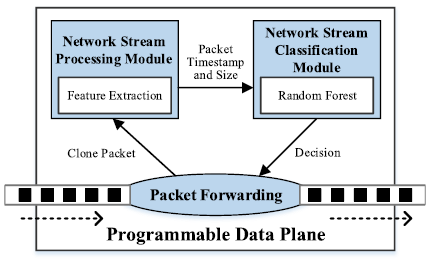
\includegraphics[width=\textwidth]{figures/fig7.png}
      \vspace{0.15cm}
      \begin{tcolorbox}[
        enhanced, boxrule=0pt,
        colback=HUApale, colframe=HUApale,
        arc=3pt, left=5pt, right=5pt,
        top=2pt, bottom=2pt,
      ]
        \centering
        \scriptsize\color{HUAdark}\itshape
        Mechanism on Defending Ransomware Attack
        with ML and PDP
      \end{tcolorbox}
    \end{column}

  \end{columns}

\end{frame}
}